\multiproblem{1}{
Consider a rod of known length $l$ and mass $m$ resting on three supports, as shown below.
            \begin{center}
                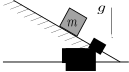
\includegraphics[scale=1.5]{fig_1.pdf}
            \end{center}
            \begin{enumerate}
            \item Draw a free-body diagram for the rod. Suppose we know that
                $N_{3}=4\newtons$. Use the external force balance and moment balance about $A$ to find the reaction forces $N_{1}$ and $N_{2}$. 
             \item Consider the case where all reaction forces at the supports are unknown. Find the external force balance and the moment balance about points $A$ and $B$. Write the system in the form ${\bf A x}={\bf b}$, where ${\bf x}=(N_{1},N_{2},N_{3})^{T}$, ${\bf A}$ is a $3\times 3$ matrix of known values and ${\bf b}$ is a $3 \times 1$ vector of known values.
             \item Construct the augmented matrix ${\bf A|b}$ and use this to solve for ${\bf x}$ and find the set of all possible values for the reaction forces $N_{1}$, $N_{2}$ and $N_{3}$. Is the system statically indeterminate?
             \item From the resting constraint $N_{i}>0$. Use this to find the minimum and maximum values of each of reaction forces.
            \end{enumerate}
}

\multiproblem{2}{
Two masses, $m_{1}$ and $m_{2}$ are connected by a spring with stiffness $k$ attached to a light inextensible string running smoothly over a pulley, as shown below.
            \begin{center}
                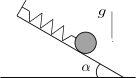
\includegraphics[scale=1.8]{fig_2.pdf}
            \end{center}
	    Mass $m_{2}$ rests on a slope at unknown angle $\theta$. 
            \begin{enumerate}
            \item Draw free body diagrams for both masses. Find the two horizontal and vertical force balance equations for each mass. 
	    \item Suppose $m_{1}$ and $m_{2}$ are known. If there is no friction acting on the slope, for which values of $\sin\theta$ is there a unique solution?
	    \item Now suppose there is friction, and that $m_{2}$, $\mu$ and $\theta$ are all known. What is the set of values of $m_{1}$ for which static equilibrium is possible? What is the corresponding extension of the spring,~$x$? Can $m_{1}=0$ and what is the condition in $\mu$ and $\theta$ for this to occur?  
	    \end{enumerate}
}

\multiproblem{3}{
A uniform rod of mass $m$ and length $L$ is connected by a pin support to the wall at one end and suspended from the wall by a light inextensible string that is attached to the other end of the rod at a known angle $\theta$, as shown below
            \begin{center}
                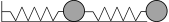
\includegraphics[scale=1.8]{fig_3.pdf}
            \end{center}
            \begin{enumerate}
	    \item Draw a free-body diagram for the rod. Assuming system is in static equilibrium, find the tension in the string.
	    \item Now find the contact force at the pin support. What angle does it make to the horizontal?
	    \end{enumerate}
}

\multiproblem{4}{
A uniform rod of mass $m$ and length $L$ learns against a wall. A mass $m_{1}$ is attached a distance $x$ from point $A$.
            \begin{center}
                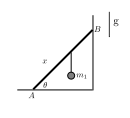
\includegraphics[scale=1.8]{fig_4.pdf}
            \end{center}
            \begin{enumerate}
	    \item Let $x=2l/3$. Draw free-body diagrams for both bodies. Assume that friction acts at $A$, with known coefficient of friction $\mu_{A}$, but not at $B$. What are the three reaction forces? What values of $\theta$ can occur for static equilibrium? 
	    \item Assume friction acts at $B$ but not $A$? Now which values of $\theta$ can occur for static equilibrium? 
	    \item Now assume that friction acts at both $A$ and $B$. Find the set of solutions for the contact forces. Is the system statically determinate? Assume it now is about to slip at $B$. What are the contact forces now?
	    \item Assume the rod is about to slip at $A$ and $B$ simultaneously. Can you find the contact forces? Allowing $m_{1}$ to be moved, where should it be placed to ensure static equilibrium?
	    \item A light inextensible string is attached to $A$ and secured to the wall. The string will break when the tension within it reaches $T_{c}$. Assuming there is no friction, how far up the rod can $m_{1}$ be placed without breaking the string? Assuming that friction acts solely at $A$, and the rod is about to slip, how far up the rod can $m_{1}$ be placed?
	    \end{enumerate}
}

\multiproblem{5}{
    Two rods are resting between two smooth walls and a smooth floor. We use a
    coorindate system that places the orign at the lower left corner of the
    room. The first rod has length $10\metres$ and mass $2m$ and rests with one end
    in the corner of the room at $(0,0)\metres$ and the other end against the
    opposite wall at $(8,6)\metres$. The second rod has length $5\metres$ and
    mass $m$ and rests between the first rod and the left-hand wall from
    $(4,3)\metres$ to $(0,6)\metres$.  The situation is shown here:
    \begin{center}
        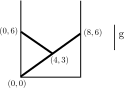
\includegraphics[scale=1.8]{fig_5.pdf}
    \end{center}
    \begin{enumerate}
        \item Given that there is no friction between the rods and the
            walls/floor find the values of all of the normal reaction forces
            between the rod/wall, rod/floor and rod/rod contacts and the value
            of the friction force between the two rods.
        \item What is the minimum value of the friction coefficient
            $\mu$ between the two rods to ensure that equilibrium is possible?
        \item Suppose we move the end of the upper rod so that it rests on a
            different part of the lower rod (but still has the same length).
            Given a particular value for the friction coefficient $\mu$ what
            possible positions can the rod-rod contact point have for
            equilibrium to occur? Are there some positions that won't work for
            any value of $\mu$?
    \end{enumerate}
}
